\section{\textit{Processor} RISC-V VeeR EL2}
\label{sub:veer-el2}

RISC-V sebagai \ac{ISA} yang \textit{open}, memiliki banyak variasi \textit{processor} yang dikembangkan oleh berbagai perusahaan maupun individu lain. \textit{Processor} VeeR EL2 \parencite{chip2024cores} adalah satu \textit{processor} yang menggunakan RISC-V \ac{ISA}. VeeR EL2 merupakan \textit{processor} yang dikembangkan oleh Chip Alliance, ilustrasi arsitektur dari \textit{processor} secara ringkas dapat dilihat pada gambar \ref{fig:veer-el2-short}.
% TODO: LAMPIRAN A

\begin{figure}[h]
	\centering
	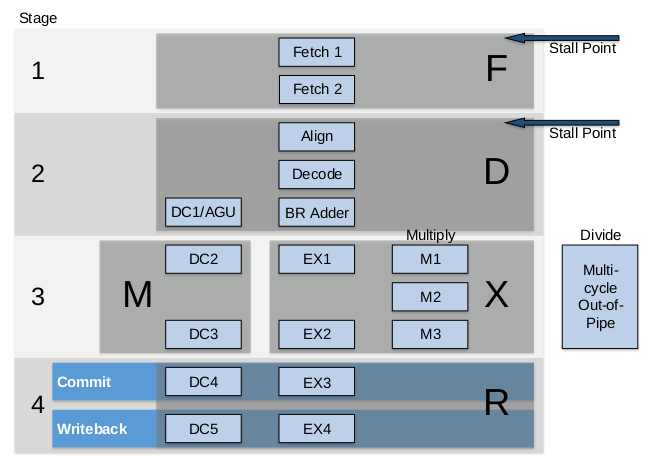
\includegraphics[width=0.8\textwidth]{chapter-2/veer-el2-short.png}
	\caption{Ilustrasi singkat arsiktektur VeeR EL2 \parencite{chip2024cores}}
	\label{fig:veer-el2-short}
\end{figure}

Deskripsi lebih detail, dari gambar \ref{fig:veer-el2-short}, arsitektur VeeR EL2 dapat terdapat pada lampiran A. Dari gambar \ref{fig:veer-el2-short}, dapat diperhatikan bahwa VeeR EL2 merupakan \textit{processor} yang miliki lima \textit{pipeline stage} sebagai berikut.

\begin{enumerate}
	\setlength{\itemsep}{0pt}
	\setlength{\parskip}{0pt}
	\item \textit{Fetch}: \textit{Stage} ketika \textit{processor} mengambil instruksi dari memori.
	\item \textit{Decode}: \textit{Stage} ketika instruksi yang diambil diidentifikasi dan disesuaikan untuk operasi pada \textit{stage} \textit{execute} dan \textit{memory}.
	\item \textit{Execute} dan \textit{Memory}: \textit{Stage} yang melakukan operasi sesuai dengan diminta oleh \textit{stage decode}.
	\item \textit{Writeback}: \textit{Stage} yang menuliskan hasil dari instruksi yang dieksekusi kembali ke register atau memori jika diperlukan.
\end{enumerate}

VeeR EL2 memiliki kelebihan fleksibilitas dalam \textit{stage execute} dan \textit{memory} yang fleksibel untuk diimplementasikan sebuah ekstensi. Hal tersebut merupakan alasan dari pemilihan VeeR EL2 sebagai \textit{processor} yang dipilih untuk implementasi ekstensi \ac{ISA} RISC-V untuk akselerator \ac{RL} pada penelitian ini.
